
\section{Технический проект}

\subsection{Общие сведения о программной системе}

Разрабатываемая компонентно-ориентированная программная система предназначена
для построения интерактивных приложений на языке Java. Система не является
прикладной программой с фиксированным набором экранов и заранее заданной
предметной областью. Ее основное назначение состоит в том, чтобы предоставить
Java-разработчику программную основу для создания собственных сцен, объектов,
компонентов, систем обработки и пользовательских сценариев поведения.

В рамках технического проекта программная система рассматривается как
легковесный движок, ориентированный на программное создание интерактивных
сцен. В составе разработки отсутствует визуальный редактор, поэтому основным
интерфейсом взаимодействия с системой является Java API. Разработчик создает
экземпляр приложения, задает конфигурацию, формирует сцену, регистрирует
системы обработки и добавляет в сцену сущности с наборами компонентов.
После запуска приложения основной цикл выполняет обновление активной сцены,
обработку пользовательского ввода, выполнение скриптов, расчет базовой физики
и отрисовку кадра.

Ключевая идея проектирования заключается в разделении объекта сцены и его
функциональных признаков. Объект сцены представлен сущностью, а его состояние
и поведение задаются компонентами. Например, объект камеры содержит компонент
\texttt{Transform}, компонент \texttt{Camera} и скрипт свободного перемещения,
а физический визуальный объект содержит \texttt{Transform}, \texttt{Rigidbody},
\texttt{BoxCollider} и \texttt{MeshRenderer}. Обработка сущностей выполняется
специализированными системами: скриптовой, физической, графической и
отладочной.

Такое устройство позволяет отказаться от глубокой иерархии классов для
разных типов объектов. Вместо классов вида 	exttt{Player}, 	exttt{Wall},
	exttt{Platform} и 	exttt{LightObject} используется сборка сущности из
небольших независимых компонентов. В результате один и тот же компонент может
переиспользоваться в разных объектах сцены, а новая функциональность добавляется
без изменения базового класса сущности. Такое решение соответствует принципам
разделения ответственности, слабой связанности, поддерживаемости и независимого
развития частей программной системы
\cite{martin-clean-architecture,fowler-refactoring,sommerville-software-engineering,pressman-software-engineering}.


Общая архитектура разрабатываемой программной системы представлена на
рисунке~\ref{fig:engine-architecture}. При оформлении проектных диаграмм учитывались рекомендации по практическому
применению UML \cite{booch-uml-guide,fowler-uml-distilled,larman-uml-patterns}.

\begin{figure}[H]
\centering
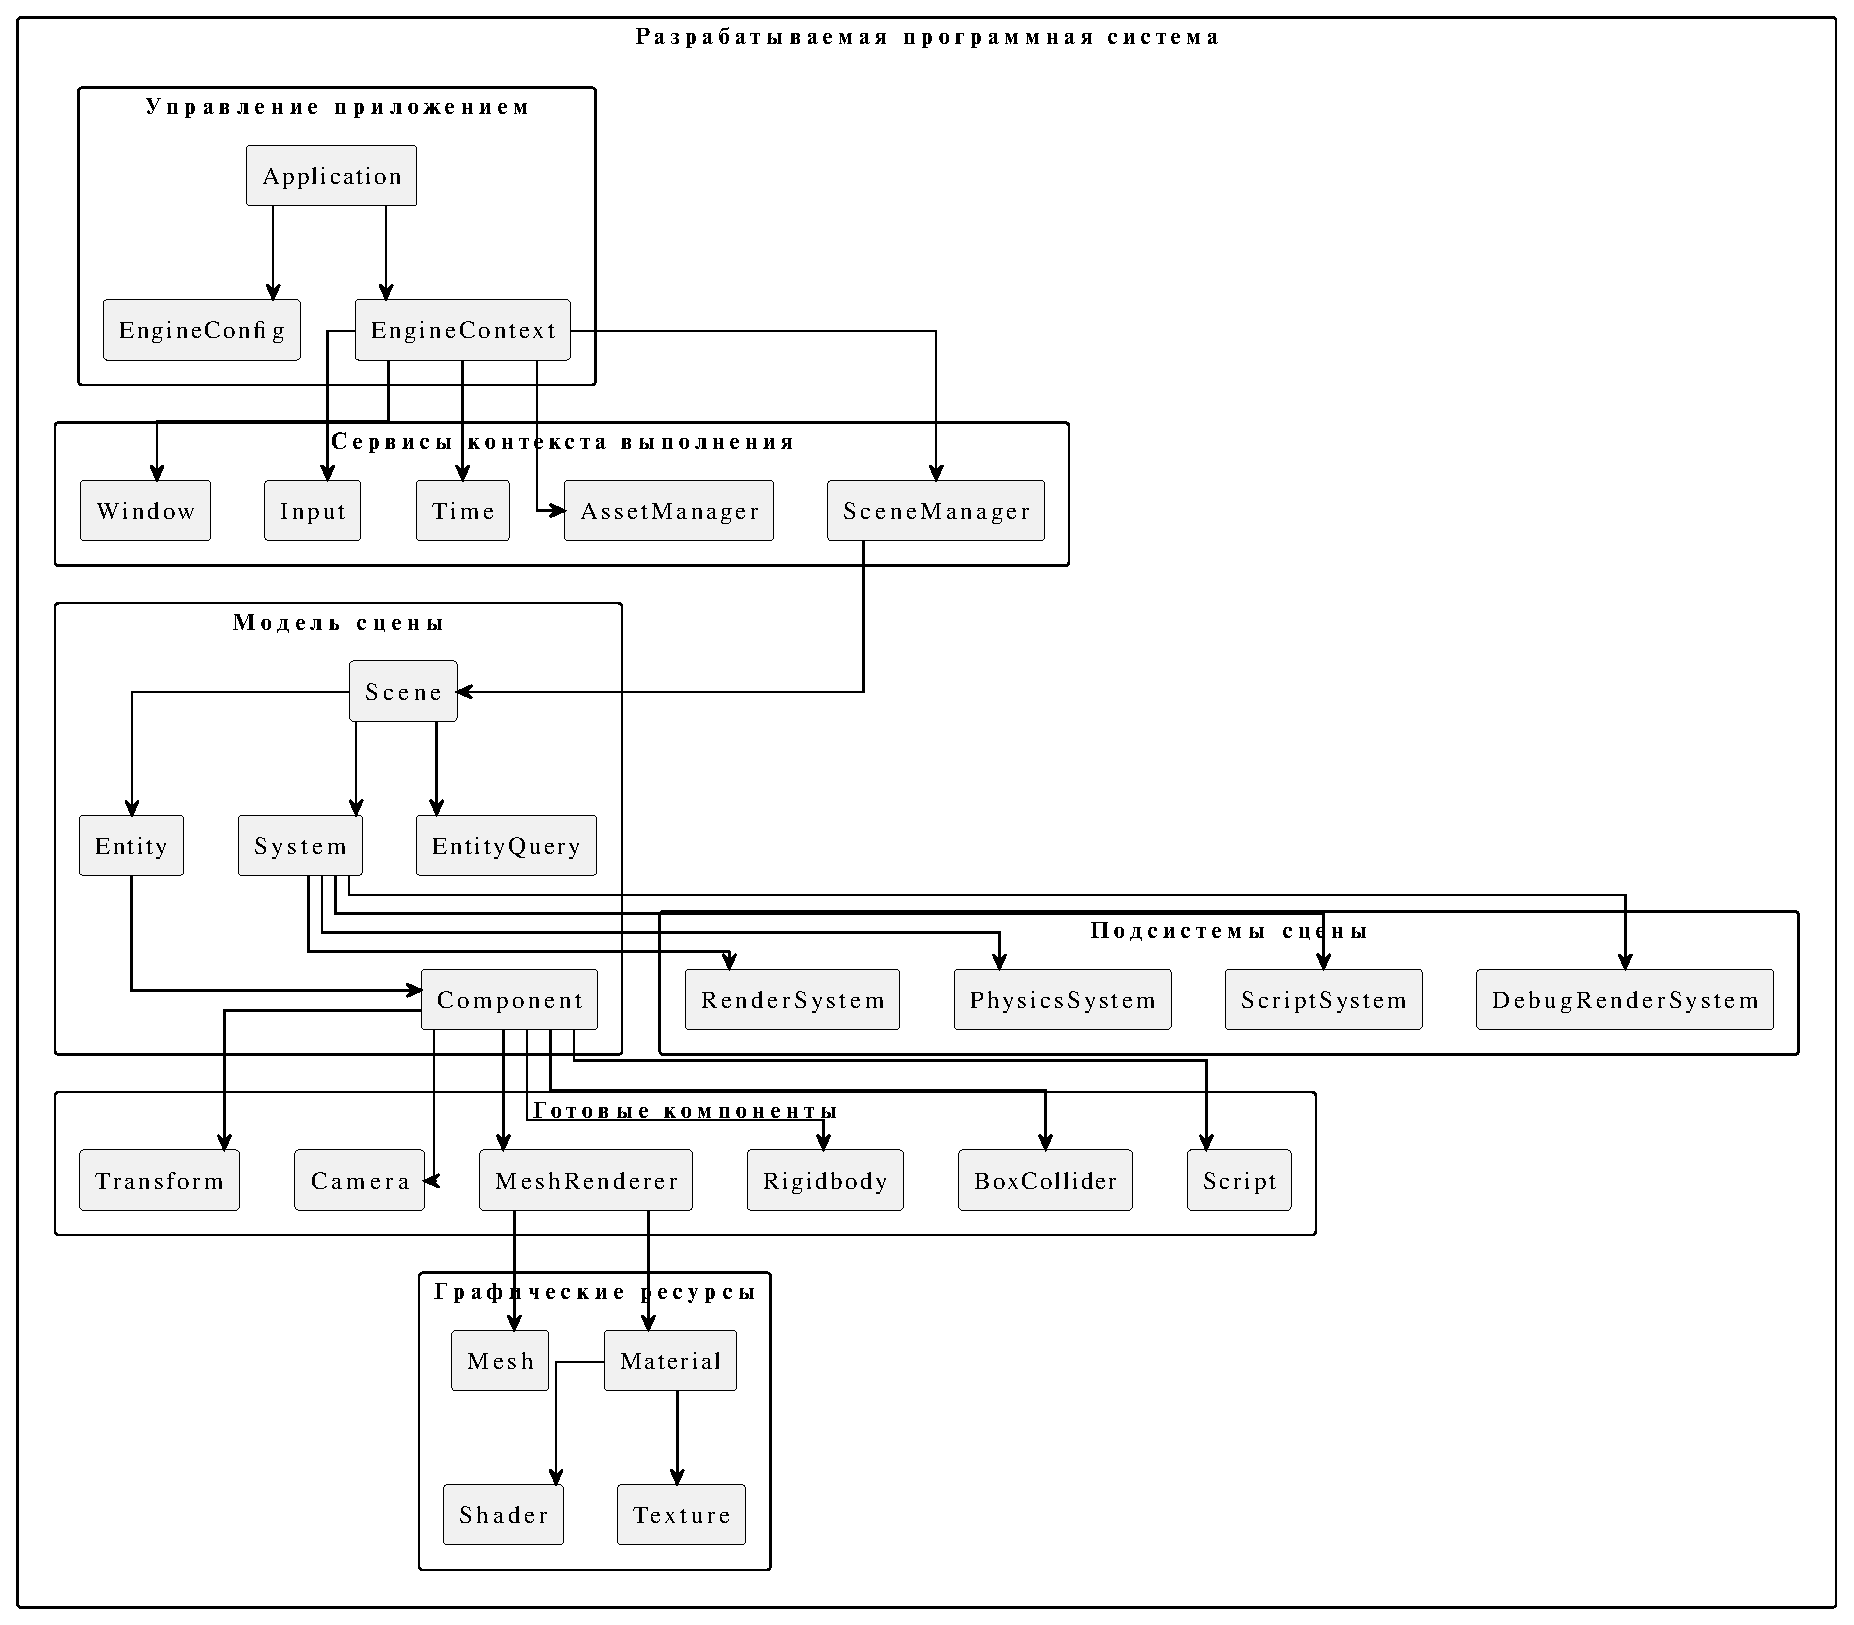
\includegraphics[width=0.95\textwidth]{images/engine-architecture.eps}
\caption{Общая архитектура программной системы}
\label{fig:engine-architecture}
\end{figure}

В дальнейшем технический проект раскрывает не проект базы данных, так как база
данных в системе не используется, а внутреннее устройство программной системы:
структуру пакетов, принципы работы сцены, жизненный цикл приложения, устройство
основных компонентов, графическую подсистему, подсистему ресурсов, скрипты,
отладочную визуализацию и самостоятельно реализованную физическую подсистему.

\subsection{Обоснование выбора технологий}

Для реализации системы выбран набор технологий, который позволяет сохранить
доступ к низкоуровневым возможностям графической подсистемы и при этом
организовать архитектуру в привычной для Java-разработчика объектной форме.
Основные технологии и их назначение приведены в таблице~\ref{tab:technologies-purpose}.

\begingroup
\small
\setlength{\tabcolsep}{4pt}
\renewcommand{\arraystretch}{1.2}

\begin{longtable}{|
>{\raggedright\arraybackslash}p{0.20\textwidth}|
>{\raggedright\arraybackslash}p{0.27\textwidth}|
>{\raggedright\arraybackslash}p{0.44\textwidth}|}
\caption{Используемые технологии и их назначение}
\label{tab:technologies-purpose}\\
\hline
\centrow Технология &
\centrow Назначение &
\centrow Причина использования \\
\hline
\endfirsthead

\multicolumn{3}{l}{Продолжение таблицы~\ref{tab:technologies-purpose}}\\
\hline
\centrow Технология &
\centrow Назначение &
\centrow Причина использования \\
\hline
\endhead

\hline
\endlastfoot

Java 25 &
основной язык реализации программной системы &
обеспечивает объектно-ориентированную модель, строгую типизацию,
кроссплатформенность на уровне JVM и удобство построения расширяемого API. \\ \hline

LWJGL 3.3.6 &
доступ из Java к нативным библиотекам &
позволяет использовать OpenGL, GLFW и STB без перехода на C/C++, при этом не
навязывает собственную архитектуру игрового движка. \\ \hline

OpenGL &
графический API для вывода сцены &
используется для создания GPU-ресурсов, передачи вершинных данных,
настройки буферов и выполнения команд отрисовки. \\ \hline

GLSL &
язык шейдерных программ &
используется для описания вершинного и фрагментного шейдеров, расчета
преобразований, текстурирования и базового освещения объектов. \\ \hline

GLFW &
создание окна, OpenGL-контекста и обработка событий ввода &
позволяет работать с настольным окном приложения, клавиатурой, мышью,
событиями изменения размера окна и состоянием курсора. \\ \hline

STB &
загрузка изображений с диска &
используется для загрузки текстур, применяемых материалами графической
подсистемы. \\ \hline

\end{longtable}
\endgroup

\subsubsection{Язык программирования Java}

Java выбрана в качестве основного языка реализации, так как архитектура системы
строится вокруг объектов, классов и интерфейсов, а сама платформа имеет
подробные спецификации языка и виртуальной машины \cite{oracle-java25,java-language-spec,java-vm-spec}.
Архитектура системы опирается на классы, наследование, инкапсуляцию и обобщенные типы. Компоненты
сцены, системы обработки, менеджеры ресурсов и пользовательские скрипты
представлены обычными Java-классами. Это делает программный интерфейс
понятным для разработчика, знакомого с объектно-ориентированным
программированием.

Дополнительным преимуществом является наличие виртуальной машины JVM.
Приложение может запускаться на разных операционных системах при наличии
установленного JDK, нативных библиотек LWJGL для целевой платформы и
графического драйвера с поддержкой требуемой версии OpenGL. Для разрабатываемой
системы это важно, поскольку она предназначена не для одной демонстрационной
сцены, а для создания разных интерактивных приложений на общей программной
основе.

\subsubsection{Библиотека LWJGL}

LWJGL используется как низкоуровневый слой доступа к нативным библиотекам \cite{lwjgl,bejarano-lwjgl,gordon-opengl-java}.
В рамках проекта задействованы GLFW, OpenGL и STB. При этом LWJGL не
определяет структуру сцены, систему компонентов, жизненный цикл приложения,
графическую очередь или физическую модель. Эти части реализуются в самой
разрабатываемой системе.

Такое разделение удобно для проектирования. С одной стороны, система получает
доступ к реальному графическому API и нативному окну. С другой стороны,
прикладной разработчик не обязан напрямую работать с повторяющимся
низкоуровневым кодом: создание окна, управление ресурсами, обновление сцены,
отрисовка и обработка ввода вынесены в отдельные классы движка.

\subsubsection{OpenGL и GLSL}

Проектирование графической подсистемы выполняется с учетом модели OpenGL,
спецификации версии 3.3 Core Profile, справочных материалов OpenGL Wiki и
спецификации GLSL 3.30 \cite{khronos-opengl,opengl-spec-33,opengl-wiki,glsl-330}.

OpenGL применяется для вывода объектов сцены \cite{khronos-opengl,opengl-spec-33,opengl-wiki,opengl-programming-guide,opengl-superbible}. На уровне графической
подсистемы создаются вершинные массивы, буферы вершин, индексные буферы и
выполняются команды отрисовки. Геометрия объекта хранится в классе
\texttt{Mesh}, а ее GPU-представление создается и кэшируется при первом
использовании в рендеринге.

Шейдеры написаны на языке GLSL. Вершинный шейдер получает данные вершины
и матрицы модели, вида и проекции. Фрагментный шейдер использует параметры
материала, текстуру, цвет и данные направленного источника света. Такой набор
достаточен для демонстрации трехмерной сцены с материалами, текстурами,
камерой и базовым направленным освещением.

\subsubsection{GLFW и STB}

Подсистема окна и ввода опирается на GLFW, а загрузка изображений выполняется
через STB \cite{glfw-docs,stb}.

GLFW используется для создания окна приложения, настройки OpenGL-контекста,
обработки событий клавиатуры, мыши, прокрутки и изменения размеров окна.
Состояние ввода сохраняется в объекте, доступном через фасад \texttt{Input},
поэтому пользовательские скрипты могут работать с клавишами и мышью без
прямого обращения к callback-функциям GLFW.

STB применяется для загрузки изображений с диска \cite{stb}. В текущей версии системы
поддержана загрузка текстур, которые затем используются материалами. Загрузка
трехмерных моделей из файлов не реализуется: геометрия задается программно,
а для типовых случаев используются встроенные примитивы.

\subsection{Внутреннее устройство программной системы}

\subsubsection{Структура пакетов проекта}

Для описания структуры проекта и зависимостей между частями используются
UML-диаграммы, подготовленные средствами PlantUML \cite{uml-spec,plantuml}.

Исходный код системы разделен на пакеты, каждый из которых отвечает за
отдельную часть архитектуры. Такое разделение позволяет отделить ядро
компонентной модели от графики, физики, управления приложением и
пользовательских скриптов. Основные пакеты проекта приведены в
таблице~\ref{tab:project-packages}.

\begingroup
\small
\setlength{\tabcolsep}{4pt}
\renewcommand{\arraystretch}{1.2}

\begin{longtable}{|
>{\raggedright\arraybackslash}p{0.24\textwidth}|
>{\raggedright\arraybackslash}p{0.27\textwidth}|
>{\raggedright\arraybackslash}p{0.40\textwidth}|}
\caption{Основные пакеты проекта}
\label{tab:project-packages}\\
\hline
\centrow Пакет &
\centrow Назначение &
\centrow Основные классы \\
\hline
\endfirsthead

\multicolumn{3}{l}{Продолжение таблицы~\ref{tab:project-packages}}\\
\hline
\centrow Пакет &
\centrow Назначение &
\centrow Основные классы \\
\hline
\endhead

\hline
\endlastfoot

\texttt{common} &
математические и вспомогательные классы &
\texttt{Vec2}, \texttt{Vec3}, \texttt{Vec4}, \texttt{Mat4}, \texttt{Quaternion}. \\ \hline

\texttt{core} &
ядро компонентно-ориентированной модели &
\texttt{Entity}, \texttt{Component}, \texttt{System}, \texttt{EntityQuery},
\texttt{EntityObserver}. \\ \hline

\texttt{engine} &
управление приложением, сценами и ресурсами &
\texttt{Application}, \texttt{EngineContext}, \texttt{EngineConfig},
\texttt{Scene}, \texttt{SceneManager}, \texttt{AssetManager}, \texttt{Input},
\texttt{Time}. \\ \hline

\texttt{component} &
готовые компоненты объектов сцены &
\texttt{Transform}, \texttt{Camera}, \texttt{MeshRenderer},
\texttt{DirectionalLight}, \texttt{Script}, \texttt{Rigidbody},
\texttt{Collider}, \texttt{BoxCollider}. \\ \hline

\texttt{graphics} &
обертки над графическими ресурсами OpenGL &
\texttt{Window}, \texttt{Shader}, \texttt{Texture}, \texttt{MeshGpuResource}. \\ \hline

\texttt{system} &
системы обработки сцены &
\texttt{ScriptSystem}, \texttt{PhysicsSystem}, \texttt{RenderSystem},
\texttt{DebugRenderSystem}. \\ \hline

\texttt{script} &
переиспользуемые пользовательские скрипты &
\texttt{FreecamController}. \\ \hline

\end{longtable}
\endgroup

Пакет \texttt{core} не зависит от OpenGL или LWJGL и содержит только общие
понятия компонентной модели. Пакеты \texttt{component} и \texttt{system}
строятся поверх ядра. Пакет \texttt{engine} объединяет инфраструктуру
приложения, а пакет \texttt{graphics} содержит классы, непосредственно связанные
с графическими ресурсами.

\subsubsection{Основные элементы внутреннего устройства}

Вместо проекта базы данных в данной работе рассматривается внутреннее устройство
программной системы. Основные элементы системы приведены в
таблице~\ref{tab:internal-elements}.

\begingroup
\small
\setlength{\tabcolsep}{4pt}
\renewcommand{\arraystretch}{1.2}

\begin{longtable}{|
>{\raggedright\arraybackslash}p{0.24\textwidth}|
>{\raggedright\arraybackslash}p{0.28\textwidth}|
>{\raggedright\arraybackslash}p{0.39\textwidth}|}
\caption{Основные элементы внутреннего устройства программной системы}
\label{tab:internal-elements}\\
\hline
\centrow Элемент &
\centrow Роль в системе &
\centrow Особенности реализации \\
\hline
\endfirsthead

\multicolumn{3}{l}{Продолжение таблицы~\ref{tab:internal-elements}}\\
\hline
\centrow Элемент &
\centrow Роль в системе &
\centrow Особенности реализации \\
\hline
\endhead

\hline
\endlastfoot

\texttt{Application} &
верхний управляющий объект приложения &
создает окно, контекст выполнения, менеджеры ресурсов и сцен, запускает основной цикл. \\ \hline

\texttt{EngineContext} &
контейнер общих сервисов &
объединяет окно, ввод, время, менеджер ресурсов, менеджер сцен и конфигурацию. \\ \hline

\texttt{Scene} &
центральный контейнер выполнения &
хранит сущности, системы, запросы, индекс компонентов и очередь отложенных изменений. \\ \hline

\texttt{Entity} &
объект сцены &
представляет именованный контейнер компонентов, сам по себе не задает поведение объекта. \\ \hline

\texttt{Component} &
признак или часть поведения сущности &
имеет ссылку на сущность и методы жизненного цикла: присоединение, запуск, остановку и уничтожение. \\ \hline

\texttt{System} &
обработчик сущностей сцены &
выполняется в заданном порядке и получает доступ к сущностям через запросы. \\ \hline

\texttt{EntityQuery} &
механизм выборки сущностей &
позволяет системе работать только с сущностями, имеющими требуемый набор компонентов. \\ \hline

\texttt{AssetManager} &
менеджер графических ресурсов &
кэширует шейдеры и текстуры, освобождает созданные ресурсы при завершении работы. \\ \hline

\end{longtable}
\endgroup

Ключевыми элементами внутреннего устройства являются \texttt{Scene},
\texttt{Entity}, \texttt{Component} и \texttt{System}. Именно они определяют
способ построения интерактивных приложений на базе разработанной системы.
Диаграмма классов ядра компонентной модели представлена на
рисунке~\ref{fig:core-class-diagram}.

\begin{figure}[H]
\centering
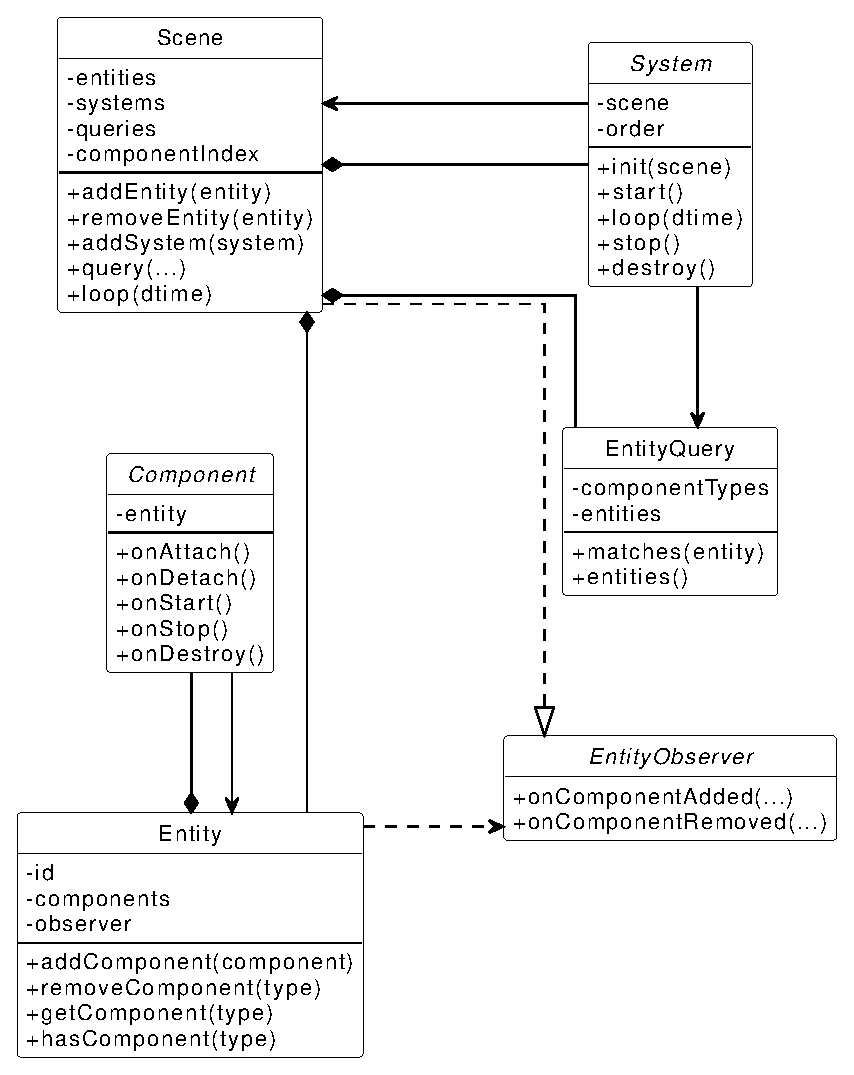
\includegraphics[width=0.95\textwidth]{images/core-class-diagram.eps}
\caption{Диаграмма классов ядра компонентной модели}
\label{fig:core-class-diagram}
\end{figure}

\subsubsection{Устройство приложения и контекста выполнения}

Класс \texttt{Application} отвечает за создание и выполнение приложения. При
создании экземпляра приложения формируется окно, создается объект
\texttt{EngineContext}, инициализируются менеджер ресурсов, менеджер сцен,
объект времени и состояние ввода. После этого разработчик загружает сцену
через \texttt{SceneManager} и вызывает метод запуска приложения.

Контекст выполнения используется для того, чтобы основные подсистемы могли
обращаться к общим сервисам. Например, пользовательский скрипт может получить
текущее состояние ввода через фасад \texttt{Input}, а графическая подсистема —
обратиться к менеджеру ресурсов. Такое решение уменьшает количество ссылок,
которые пришлось бы вручную передавать между скриптами, системами и сценами.

Конфигурация приложения вынесена в отдельный объект \texttt{EngineConfig}.
В ней задаются параметры, влияющие на выполнение приложения: цвет очистки
окна, фиксированный шаг времени, масштаб времени, автоматическое обновление
соотношения сторон камер и режим проверки ошибок OpenGL. Благодаря этому
настройки не смешиваются с логикой сцены.

\subsubsection{Устройство сцены}

Сцена является центральной частью выполнения интерактивного приложения.
Внутри нее хранятся сущности, системы обработки, запросы сущностей, индекс
компонентов и очередь отложенных структурных изменений. Такое устройство
необходимо потому, что во время выполнения кадра состав сцены может меняться:
скрипт может создать новый объект, удалить существующий, добавить компонент
или запросить изменение активной сцены.

Сцена хранит сущности в отображении по строковому идентификатору. Это
позволяет быстро получать объект по имени и не допускать добавления двух
сущностей с одинаковым идентификатором. Системы обработки хранятся отдельно
и сортируются по числовому порядку выполнения. Благодаря этому можно явно
задавать, что система скриптов должна обновляться раньше физики, физика —
раньше рендеринга, а отладочная отрисовка — после основной отрисовки сцены.

Для ускорения поиска объектов сцена поддерживает индекс компонентов. При
добавлении сущности каждый ее компонент заносится в индекс. При удалении
сущности или компонента индекс обновляется. Запрос \texttt{EntityQuery} содержит
набор требуемых компонентов и хранит множество сущностей, удовлетворяющих
этому набору. Например, графическая система создает запрос по компонентам
\texttt{Transform} и \texttt{MeshRenderer}, а физическая система — запросы по
\texttt{Transform}, \texttt{Rigidbody} и наследникам \texttt{Collider}.

Отдельное значение имеет механизм отложенных структурных изменений. Если
сцена в данный момент выполняет системы, немедленное добавление или удаление
объекта может нарушить обход коллекций. Поэтому при обновлении сцены такие
изменения помещаются в очередь. После завершения текущего прохода систем
очередь применяется в безопасный момент. В результате пользовательские скрипты
могут менять состав сцены, не создавая ошибок обхода и не нарушая согласованное
состояние запросов.

При запуске сцена инициализирует сущности, строит индексы, перестраивает
запросы и вызывает метод \texttt{init} у систем. Затем запускаются компоненты
сущностей и системы обработки. При остановке сцены системы останавливаются,
после чего останавливаются компоненты. При уничтожении сцены освобождаются
системы, сущности, индексы и запросы.

\subsubsection{Сущности, компоненты и системы обработки}

При проектировании ядра компонентной модели учитывались как классические
подходы объектно-ориентированного проектирования, так и практические материалы
по компонентным объектным системам \cite{gamma-patterns,bilas-object-system,west-hierarchy}.

Сущность представляет собой именованный контейнер компонентов. Она не содержит
собственной прикладной логики и не наследуется от конкретных классов объектов.
Смысл сущности определяется тем, какие компоненты к ней добавлены. Компонент
\texttt{Transform} задает пространственное положение, \texttt{Camera} делает
объект камерой, \texttt{MeshRenderer} позволяет отрисовать объект,
\texttt{Rigidbody} включает объект в физическое моделирование, а наследник
\texttt{Script} добавляет пользовательское поведение.

Базовый класс \texttt{Component} имеет жизненный цикл. При добавлении к сущности
компонент получает ссылку на нее и может выполнить логику присоединения. При
запуске сцены вызываются методы запуска, при остановке — методы остановки, при
удалении — методы уничтожения. Это важно для компонентов, которые используют
внутренние ресурсы или должны корректно реагировать на изменение состояния
сцены.

Система обработки является объектом, который выполняется каждый кадр и
работает с выбранными сущностями. В отличие от компонента, система обычно не
принадлежит одной конкретной сущности. Она рассматривает сцену целиком и
выбирает объекты по составу компонентов. Например, \texttt{RenderSystem} не
хранится в каждом визуальном объекте, а обходит все сущности с компонентами
\texttt{Transform} и \texttt{MeshRenderer}. Такой подход уменьшает связанность
между объектами и централизует обработку однотипной логики.

\subsubsection{Жизненный цикл приложения и сцены}

Жизненный цикл одного кадра строится вокруг активной сцены. На каждом кадре
приложение очищает окно, обновляет время, вызывает обновление активной сцены,
применяет отложенные изменения, обновляет параметры камер, состояние ввода и
окно. Последовательность выполнения одного кадра представлена на
рисунке~\ref{fig:frame-lifecycle}.

\begin{figure}[H]
\centering
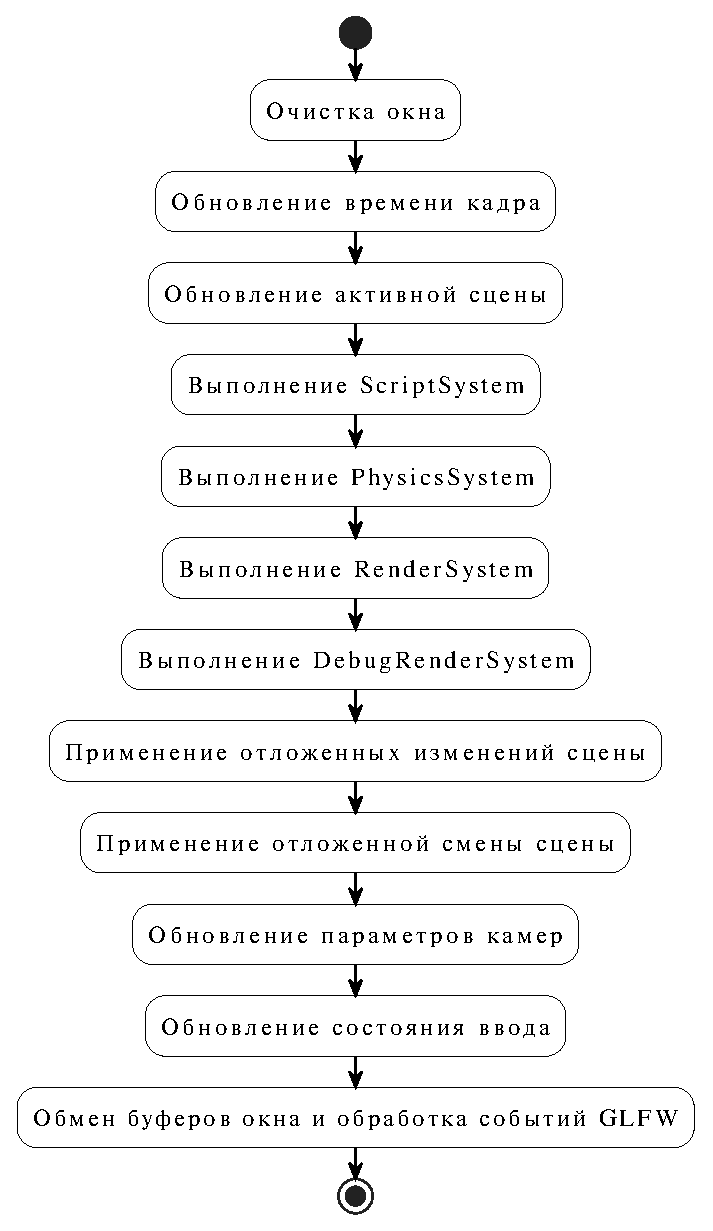
\includegraphics[width=0.85\textwidth]{images/frame-lifecycle.eps}
\caption{Последовательность выполнения одного кадра приложения}
\label{fig:frame-lifecycle}
\end{figure}

Внутри обновления сцены выполняются зарегистрированные системы. Порядок
выполнения задается числовым приоритетом системы. Для интерактивных сцен
используется последовательность, при которой сначала выполняется
\texttt{ScriptSystem}, затем \texttt{PhysicsSystem}, далее \texttt{RenderSystem}
и \texttt{DebugRenderSystem}. Такой порядок выбран не случайно: скрипт может
изменить управление объектом, физика обновляет положение тел, а рендеринг
отображает уже обновленное состояние сцены.

\subsection{Проектирование основных подсистем}

\subsubsection{Подсистема управления сценами}

Управление сценами выполняет \texttt{SceneManager}. Он хранит активную сцену и
поддерживает операции загрузки, замены, отложенной загрузки и отложенной замены.
При обычной загрузке старая сцена останавливается, а новая инициализируется и
запускается. При замене старая сцена дополнительно уничтожается.

Отложенная замена нужна для случаев, когда команда смены сцены вызывается из
системы или пользовательского скрипта во время кадра. Например, обработчик перезапуска демонстрационной сцены может запросить
создание новой сцены. Немедленное
уничтожение текущей сцены в середине обновления было бы опасным, поэтому
менеджер сцен применяет такое изменение после завершения текущего кадра.

\subsubsection{Графическая подсистема}

Графическая подсистема разрабатывается как слой между компонентами сцены и
низкоуровневым графическим API. При проектировании учитывались подходы к
рендерингу в реальном времени и практические руководства по OpenGL
\cite{realtime-rendering,eberly-engine,lengyel-rendering,opengl-programming-guide,opengl-superbible}.

Графическая подсистема отвечает за отображение сцены средствами OpenGL. Ее
центральным классом является \texttt{RenderSystem}. При инициализации система
создает три запроса: к отрисовываемым объектам, к камерам и к направленным
источникам света. Отрисовываемыми считаются сущности, имеющие компоненты
\texttt{Transform} и \texttt{MeshRenderer}. Камерами считаются сущности с
\texttt{Transform} и \texttt{Camera}. Направленное освещение задается компонентом
\texttt{DirectionalLight}.

На каждом кадре \texttt{RenderSystem} сначала выбирает активную камеру. Если
в сцене присутствует несколько камер, выбирается включенная камера с наибольшим
приоритетом. Затем выбирается активный направленный источник света. После
этого строится очередь команд отрисовки: система обходит все сущности с
\texttt{Transform} и \texttt{MeshRenderer}, проверяет наличие меша и материала,
активность рендерера, соответствие слоя объекта маске камеры и видимость
объекта относительно текущей камеры.

Видимость объекта проверяется по ограничивающей сфере. Радиус этой сферы
хранится в \texttt{MeshRenderer}. Объект переводится в пространство камеры,
после чего отбрасывается, если находится за ближней или дальней плоскостью
отсечения либо выходит за границы области видимости камеры с учетом радиуса.
Для ортографической и перспективной камеры используются разные расчеты границ,
но общий смысл одинаков: объект, не попадающий в область обзора, не добавляется
в очередь отрисовки.

После построения очередь сортируется. В системе используется сортировка по
очереди рендеринга, идентификатору шейдера, идентификатору текстуры и объекту
меша. Это уменьшает количество переключений графического состояния и делает
отрисовку более предсказуемой. Данная оптимизация не является полноценным
пакетированием графических команд, но она уже снижает число лишних смен
шейдера, текстуры и вершинных данных.

Для каждой команды отрисовки система получает GPU-представление меша.
Если меш используется впервые, создается \texttt{MeshGpuResource}, включающий
VAO, VBO и EBO. Если ресурс уже создан и версия меша не изменилась, он
переиспользуется. Если версия меша изменилась, старый GPU-ресурс уничтожается
и создается новый. Благодаря этому геометрия не загружается в видеопамять на
каждом кадре.

Перед вызовом OpenGL-команды отрисовки материал активирует шейдер и текстуру.
Затем в шейдер передаются матрицы модели, вида и проекции, параметры
направленного света, ambient-цвет и флаг наличия освещения. После этого
привязывается VAO и вызывается \texttt{glDrawElements} с режимом
\texttt{GL\_TRIANGLES}. Таким образом, каждый визуальный объект проходит путь:
сущность сцены, компоненты \texttt{Transform} и \texttt{MeshRenderer}, команда
рендеринга, GPU-ресурс меша, шейдер и команда OpenGL.

Основные классы графической подсистемы приведены в таблице
\ref{tab:graphics-classes}.

\begingroup
\small
\setlength{\tabcolsep}{4pt}
\renewcommand{\arraystretch}{1.2}

\begin{longtable}{|
>{\raggedright\arraybackslash}p{0.23\textwidth}|
>{\raggedright\arraybackslash}p{0.30\textwidth}|
>{\raggedright\arraybackslash}p{0.38\textwidth}|}
\caption{Основные классы графической подсистемы}
\label{tab:graphics-classes}\\
\hline
\centrow Класс &
\centrow Назначение &
\centrow Особенности реализации \\
\hline
\endfirsthead

\multicolumn{3}{l}{Продолжение таблицы~\ref{tab:graphics-classes}}\\
\hline
\centrow Класс &
\centrow Назначение &
\centrow Особенности реализации \\
\hline
\endhead

\hline
\endlastfoot

\texttt{RenderSystem} &
отрисовка объектов сцены &
выбирает камеру и свет, строит и сортирует очередь рендеринга, вызывает OpenGL-команды. \\ \hline

\texttt{MeshRenderer} &
визуальное представление сущности &
связывает объект сцены с мешем, материалом, слоем, очередью рендеринга и радиусом видимости. \\ \hline

\texttt{Camera} &
описание камеры &
задает перспективную или ортографическую проекцию, приоритет, маску слоев, ближнюю и дальнюю плоскости отсечения. \\ \hline

\texttt{Material} &
параметры отрисовки &
содержит шейдер, цвет, текстуру и дополнительные uniform-параметры. \\ \hline

\texttt{Mesh} &
геометрия объекта &
хранит вершины, индексы и версию данных для контроля актуальности GPU-ресурса. \\ \hline

\texttt{MeshGpuResource} &
GPU-представление меша &
содержит идентификаторы VAO, VBO, EBO и количество индексов. \\ \hline

\texttt{Shader} &
шейдерная программа &
компилирует вершинный и фрагментный шейдеры и передает uniform-переменные. \\ \hline

\texttt{Texture} &
текстура OpenGL &
загружает изображение через STB или создает отладочную текстуру. \\ \hline

\end{longtable}
\endgroup

\subsubsection{Подсистема ресурсов}

Подсистема ресурсов представлена классом \texttt{AssetManager}. Он хранит
загруженные шейдеры и текстуры в отображениях по строковому ключу. При повторном
запросе ресурса с тем же ключом возвращается уже созданный объект. Это исключает
повторную компиляцию одного и того же шейдера и повторную загрузку одной и той
же текстуры.

Менеджер ресурсов также предоставляет базовый шейдер и отладочную текстуру.
Базовый шейдер используется как стандартный вариант для материалов, которым
не задана отдельная шейдерная программа. Отладочная текстура позволяет показать
объект даже в тех случаях, когда разработчик не назначил собственную текстуру.
При завершении работы приложения \texttt{AssetManager} освобождает все созданные
шейдеры и текстуры.

\subsubsection{Подсистема пользовательского ввода}

Подсистема ввода получает события от GLFW и сохраняет их в состоянии ввода.
Поддерживаются клавиатура, кнопки мыши, положение курсора, смещение мыши и
прокрутка. Прикладной код обращается к этим данным через фасад \texttt{Input},
поэтому пользовательские скрипты не зависят от конкретной реализации callback-функций
окна.

Примером использования подсистемы ввода является \texttt{FreecamController}.
Он перемещает камеру по клавишам \texttt{W}, \texttt{A}, \texttt{S}, \texttt{D},
\texttt{SPACE} и \texttt{LEFT\_SHIFT}, а поворот камеры определяет по смещению
мыши. Такой скрипт одновременно проверяет работу ввода, трансформации и камеры.

\subsubsection{Подсистема пользовательских скриптов}

Пользовательские сценарии поведения реализуются через наследование от класса
\texttt{Script}. Так как \texttt{Script} является компонентом, он добавляется к
сущности так же, как \texttt{Camera}, \texttt{MeshRenderer} или \texttt{Rigidbody}.
Система \texttt{ScriptSystem} находит компоненты-наследники \texttt{Script} и
вызывает их методы жизненного цикла: \texttt{init}, \texttt{start}, \texttt{loop},
\texttt{stop}, \texttt{destroy}.

Скрипт может получать доступ к другим компонентам своей сущности и изменять их
состояние. Например, скрипт движущейся платформы получает \texttt{Rigidbody}
и задает ему скорость, а скрипт управления сценой отслеживает нажатие клавиши и
запрашивает перезапуск демонстрационной сцены через \texttt{SceneManager}.

\subsubsection{Подсистема отладочной визуализации}

Подсистема отладочной визуализации предназначена для вывода вспомогательной
геометрии поверх основной сцены. Она включает \texttt{DebugRenderer} и
\texttt{DebugRenderSystem}. Разработчик или другая подсистема может добавить
линии в очередь отладочной отрисовки, после чего \texttt{DebugRenderSystem}
выводит их средствами OpenGL.

В физической демонстрационной сцене отладочная визуализация используется для
сетки и границ коллайдеров. Это помогает проверять соответствие визуальной
геометрии и физической формы объекта. Подсистема не заменяет основную графику,
а служит инструментом разработки и проверки поведения сцены.

\subsection{Проектирование физической подсистемы}

Проектирование физической подсистемы основано на упрощенной модели твердых
тел, обнаружении пересечений коробочных коллайдеров и импульсном разрешении
контактов. Базовые алгоритмы таких подсистем рассматриваются в литературе по
физическому моделированию и обнаружению столкновений
\cite{ericson-collision,millington-physics,bergen-collision,mirtich-impulse,catto-iterative-dynamics,box2d-docs}.

\subsubsection{Общая структура физической подсистемы}

Физическая подсистема проектируется как самостоятельная часть системы, без
использования готового физического движка. Она предназначена для базовой
демонстрации движения твердых тел и обработки столкновений в интерактивной
сцене. В текущей версии системы
поддерживаются динамические, статические и кинематические тела, гравитация,
силы, моменты сил, линейная и угловая скорость, демпфирование, упругость,
трение, слои столкновений, маски столкновений и коллайдер типа \texttt{BoxCollider}.

Название \texttt{BoxCollider} в тексте работы следует понимать как
коллайдер формы параллелепипеда, то есть ориентированный ограничивающий
параллелепипед. Его положение, ориентация и масштаб вычисляются на основе
матрицы модели компонента \texttt{Transform}. В отличие от осево-ориентированной
границы, такой коллайдер может поворачиваться вместе с объектом сцены.

Основные классы физической подсистемы приведены в таблице
\ref{tab:physics-classes}.

\begingroup
\small
\setlength{\tabcolsep}{4pt}
\renewcommand{\arraystretch}{1.2}

\begin{longtable}{|
>{\raggedright\arraybackslash}p{0.23\textwidth}|
>{\raggedright\arraybackslash}p{0.30\textwidth}|
>{\raggedright\arraybackslash}p{0.38\textwidth}|}
\caption{Основные классы физической подсистемы}
\label{tab:physics-classes}\\
\hline
\centrow Класс &
\centrow Назначение &
\centrow Особенности реализации \\
\hline
\endfirsthead

\multicolumn{3}{l}{Продолжение таблицы~\ref{tab:physics-classes}}\\
\hline
\centrow Класс &
\centrow Назначение &
\centrow Особенности реализации \\
\hline
\endhead

\hline
\endlastfoot

\texttt{PhysicsSystem} &
расчет физики и столкновений &
использует фиксированный шаг, аккумулятор времени, итерации решения скоростей и позиций. \\ \hline

\texttt{Rigidbody} &
физическое тело &
хранит массу, обратную массу, скорость, угловую скорость, силу, момент силы, тип тела и параметры демпфирования. \\ \hline

\texttt{Collider} &
базовый класс области столкновения &
задает смещение, слой, маску столкновений, трение, упругость, флаг триггера и активность. \\ \hline

\texttt{BoxCollider} &
коллайдер формы параллелепипеда &
хранит половинные размеры по трем осям и используется для построения коллайдера формы параллелепипеда. \\ \hline

\texttt{PhysicsBodyType} &
тип физического тела &
разделяет тела на динамические, статические и кинематические. \\ \hline

\end{longtable}
\endgroup

Физическая система при инициализации создает два запроса: один для сущностей
с \texttt{Transform} и \texttt{Rigidbody}, второй для сущностей с \texttt{Transform}
и наследниками \texttt{Collider}. На каждом кадре она накапливает прошедшее
время и выполняет один или несколько физических подшагов фиксированной длины.
Число подшагов ограничивается параметром \texttt{maxSubSteps}, чтобы длинный
кадр не приводил к бесконечной попытке ``догнать'' время моделирования.

\subsubsection{Математическая модель движения}

Поступательное движение динамического тела описывается классическими
дифференциальными уравнениями движения материальной точки:

\[
\frac{d\mathbf{x}}{dt}=\mathbf{v},\qquad
\frac{d\mathbf{v}}{dt}=\mathbf{a},\qquad
\mathbf{a}=\frac{\mathbf{F}}{m}+s_g\mathbf{g},
\]

где \(\mathbf{x}\) -- положение тела, \(\mathbf{v}\) -- линейная скорость,
\(\mathbf{a}\) -- ускорение, \(\mathbf{F}\) -- сумма внешних сил, \(m\) -- масса
тела, \(\mathbf{g}\) -- вектор гравитации, \(s_g\) -- коэффициент влияния
гравитации для конкретного тела.

Для вращательного движения используется угловая скорость
\(\boldsymbol{\omega}\) и момент силы \(\boldsymbol{\tau}\):
\[
\frac{d\boldsymbol{\omega}}{dt}=\mathbf{I}^{-1}\boldsymbol{\tau},
\]

где \(\mathbf{I}\) -- тензор инерции тела. Для тела с параллелепипедным
коллайдером в коде используется приближение инерции прямоугольного
параллелепипеда. Если ширина, высота и глубина равны \(w\), \(h\) и \(d\), то
главные моменты инерции вычисляются как:
\[
I_x=\frac{m}{12}(h^2+d^2),\qquad
I_y=\frac{m}{12}(w^2+d^2),\qquad
I_z=\frac{m}{12}(w^2+h^2).
\]

В реализации хранится не сам тензор инерции, а применяется обратная инерция
по локальным осям параллелепипеда. Это нужно при расчете углового изменения
скорости от импульса, приложенного не в центре масс.

\subsubsection{Метод численного интегрирования}

Физика обновляется с фиксированным шагом \(\Delta t\). В проектном решении
для демонстрационных сцен используется шаг \(1/60\) секунды. Внутри одного физического шага сначала
обновляются скорости по силам, затем по обновленным скоростям изменяются
положение и поворот объекта. Такой порядок соответствует полуявному методу
Эйлера:

\[
\mathbf{v}_{n+1}=\mathbf{v}_{n}+\mathbf{a}_{n}\Delta t,
\qquad
\mathbf{x}_{n+1}=\mathbf{x}_{n}+\mathbf{v}_{n+1}\Delta t.
\]

Для угловой скорости используется аналогичная схема:
\[
\boldsymbol{\omega}_{n+1}=\boldsymbol{\omega}_{n}+\mathbf{I}^{-1}\boldsymbol{\tau}_{n}\Delta t.
\]

После этого из угловой скорости вычисляется малый поворот за текущий шаг:
\[
\Delta \varphi = |\boldsymbol{\omega}_{n+1}|\Delta t.
\]

Ось поворота определяется нормированным вектором угловой скорости, после чего
создается кватернион дополнительного поворота. Новый поворот объекта получается
умножением текущего кватерниона на кватернион приращения с последующей
нормализацией. Такой способ удобен для трехмерной сцены, так как позволяет
избежать проблем с накоплением углов Эйлера.

Перед применением скорости используются линейное и угловое демпфирование:
\[
\mathbf{v}_{n+1}=\mathbf{v}_{n+1}\max(0,1-k_l\Delta t),
\qquad
\boldsymbol{\omega}_{n+1}=\boldsymbol{\omega}_{n+1}\max(0,1-k_a\Delta t),
\]

где \(k_l\) -- коэффициент линейного демпфирования, а \(k_a\) -- коэффициент
углового демпфирования. Также в системе ограничиваются максимальная линейная
и максимальная угловая скорости. Это уменьшает вероятность неустойчивого
поведения при больших силах или ошибочно заданных параметрах сцены.

\subsubsection{Обнаружение столкновений}

Для проверки пересечений выпуклых коробочных форм применяется подход, близкий
к методу разделяющих осей; иерархии и ограничивающие объемы широко применяются
для ускорения таких проверок \cite{gottschalk-obbtree}.

Обнаружение столкновений состоит из двух этапов. На первом этапе выполняется
быстрая проверка пересечения осево-ориентированных ограничивающих объемов
(AABB). Если эти объемы не пересекаются, более точная проверка не выполняется.
Такой этап нужен для раннего отбрасывания пар объектов, которые находятся далеко
друг от друга.

На втором этапе для двух коллайдеров формы параллелепипеда используется проверка
по теореме разделяющих осей. Каждый \texttt{BoxCollider} преобразуется в
коллайдер формы параллелепипеда: вычисляются центр, три
локальные оси в мировых координатах и половинные размеры с учетом масштаба
объекта. Далее проверяются оси первого параллелепипеда, оси второго
параллелепипеда и попарные векторные произведения этих осей. Всего для пары
трехмерных параллелепипедов рассматривается до пятнадцати осей.

Для каждой оси вычисляются радиусы проекции двух параллелепипедов и расстояние
между их центрами вдоль этой оси. Если сумма радиусов меньше расстояния между
центрами, между объектами существует разделяющая ось, и столкновения нет. Если
пересечение найдено по всем осям, пара считается сталкивающейся. Ось с минимальным
перекрытием используется как нормаль столкновения, а величина перекрытия -- как
глубина проникновения.

После определения нормали и глубины проникновения формируется набор контактных
точек. Для этого вершины, близкие к контактной плоскости, проецируются на эту
плоскость и проверяются на принадлежность второму параллелепипеду. Если точек
получается слишком много, они сокращаются до ограниченного количества, чтобы
решатель столкновений не выполнял лишнюю работу.

\subsubsection{Разрешение столкновений}

Разрешение столкновений выполняется итерационно. Сначала несколько раз
обрабатываются скорости, затем несколько раз выполняется позиционная коррекция.
Такой подход не дает идеального аналитического решения для всех контактов сразу,
но хорошо подходит для интерактивной демонстрационной сцены.

Для контактной точки вычисляется относительная скорость:
\[
\mathbf{v}_{rel}=(\mathbf{v}_b+\boldsymbol{\omega}_b\times\mathbf{r}_b)-
(\mathbf{v}_a+\boldsymbol{\omega}_a\times\mathbf{r}_a),
\]

где \(\mathbf{r}_a\) и \(\mathbf{r}_b\) -- радиус-векторы от центра масс тел до
контактной точки. Проекция этой скорости на нормаль контакта показывает,
сближаются ли тела вдоль нормали.

Нормальный импульс вычисляется по формуле:

\[
j_n=\frac{b-\mathbf{v}_{rel}\cdot\mathbf{n}}
{m_a^{-1}+m_b^{-1}+D_a+D_b},
\]

где \(\mathbf{n}\) -- нормаль контакта, \(b\) -- скоростная поправка, учитывающая
упругость и баумгартовскую коррекцию проникновения, \(D_a\) и \(D_b\) --
угловые добавки, возникающие из-за приложения импульса не в центре масс.
Если знаменатель равен нулю или тела не должны двигаться, импульс не применяется.

После нормального импульса рассчитывается касательное направление и импульс
трения. Его величина ограничивается максимальным значением, пропорциональным
нормальному импульсу и коэффициенту трения. Благодаря этому объект может не
только отскакивать от поверхности, но и постепенно терять касательную скорость
при контакте.

Позиционная коррекция устраняет остаточное взаимное проникновение тел. В
системе используется небольшая допустимая глубина \(s\), после которой часть
проникновения распределяется между телами пропорционально обратным массам:
\[
C=\min(0{,}05,\max(0,p-s)\cdot 0{,}2),
\]

где \(p\) -- глубина проникновения. Если одно тело статическое, вся коррекция
фактически приходится на динамическое тело. Такой способ не делает физику
абсолютно точной, но предотвращает заметное накопление проникновений между
объектами.

\subsubsection{Архитектурные ограничения физической подсистемы}

Физическая подсистема предназначена для базовой обработки твердых тел и
столкновений в демонстрационных интерактивных сценах. На текущем этапе
поддерживается параллелепипедный тип коллайдера, динамические, статические и
кинематические тела, импульсное разрешение столкновений, трение, упругость,
ограничение скорости и режим сна для устойчиво покоящихся тел.

При этом система не ставит целью заменить промышленный физический движок. В
текущую область разработки не входят составные соединения тел, шарнирные
ограничители, непрерывное обнаружение столкновений для очень быстрых объектов,
коллайдеры произвольной сетки и сложные материалы. Такое ограничение соответствует
задачам ВКР: необходимо показать собственную архитектуру физической подсистемы
и ее совместную работу со сценой, компонентами, скриптами и рендерингом.


\subsection{Проектирование демонстрационных сцен}

Для проверки применимости архитектуры к разным типам интерактивных приложений
в проекте предусматривается не одна, а несколько демонстрационных сцен. Каждая
сцена строится программно средствами Java API и использует общий набор элементов:
сущности, компоненты, системы обработки, ресурсы, пользовательские скрипты и
жизненный цикл сцены. Отличие сцен состоит в том, какие подсистемы они делают
основными и какие сценарии взаимодействия должны быть проверены после реализации.

На стадии технического проектирования демонстрационные сцены рассматриваются как
проектные сценарии применения движка. Они не заменяют системное тестирование:
скриншоты, пошаговые проверки и фактические результаты работы сцен должны быть
приведены в рабочем проекте. В данном разделе фиксируется назначение сцен и их
роль в подтверждении выбранной архитектуры.

Состав демонстрационных сцен приведен в таблице~\ref{tab:demo-scenes-design}.

\begingroup
\small
\setlength{\tabcolsep}{4pt}
\renewcommand{\arraystretch}{1.2}

\begin{longtable}{|
>{\raggedright\arraybackslash}p{0.22\textwidth}|
>{\raggedright\arraybackslash}p{0.32\textwidth}|
>{\raggedright\arraybackslash}p{0.37\textwidth}|}
\caption{Проектное назначение демонстрационных сцен}
\label{tab:demo-scenes-design}\\
\hline
\centrow Сцена &
\centrow Основные подсистемы &
\centrow Проектное назначение \\
\hline
\endfirsthead

\multicolumn{3}{l}{Продолжение таблицы~\ref{tab:demo-scenes-design}}\\
\hline
\centrow Сцена &
\centrow Основные подсистемы &
\centrow Проектное назначение \\
\hline
\endhead

\hline
\endlastfoot

\texttt{ShowcaseScene} &
сцена, трансформации, камера, освещение, рендеринг, отладочная визуализация &
демонстрация базовой трехмерной сцены, иерархии объектов, свободной камеры,
направленного света, слоев видимости, направляющих и ограничивающих объемов. \\ \hline

\texttt{Interactive2DScene} &
ортографическая камера, ввод мыши, пользовательские скрипты, 2D-представление
объектов &
демонстрация интерактивного сценария с обработкой положения курсора, нажатий
мыши, переключателей, изменения цвета, вращения, пульсации и слайдера. \\ \hline

\texttt{TexturedLightingScene} &
материалы, текстуры, шейдеры, направленное освещение, скрипты анимации &
демонстрация работы материалов, процедурно созданных и загружаемых текстур,
передачи uniform-параметров в шейдеры и изменения источника света во времени. \\ \hline

\texttt{PhysicsScene} &
физика, коллайдеры, динамические и кинематические тела, рендеринг,
отладочная визуализация &
демонстрация совместной работы физической подсистемы, визуального отображения,
скриптов управления, перезапуска сцены и отладочного отображения границ
коллайдеров. \\ \hline

\end{longtable}
\endgroup

Набор сцен выбран так, чтобы не сводить проверку программной системы к одному
частному примеру. \texttt{ShowcaseScene} подтверждает базовую пригодность
архитектуры для трехмерной сцены. \texttt{Interactive2DScene} показывает, что
та же компонентная модель применима для интерактивных двумерных объектов и
обработки пользовательского ввода. \texttt{TexturedLightingScene} выделяет
графическую часть, связанную с материалами, текстурами и освещением.
\texttt{PhysicsScene} используется как наиболее комплексный сценарий, в котором
одновременно задействованы сцена, скрипты, рендеринг, ввод, физика и отладочная
визуализация.

При проектировании демонстрационных сцен приняты следующие общие решения:
сцены создаются программно без визуального редактора; каждая сцена регистрирует
собственный набор систем обработки; объекты сцены формируются из сущностей и
компонентов; повторяющиеся элементы поведения выносятся в пользовательские
скрипты; переключение или перезапуск сцены выполняется через \texttt{SceneManager}
с учетом механизма отложенных структурных изменений.

\subsection{Выводы по разделу}

В рамках технического проекта определено внутреннее устройство разрабатываемой
компонентно-ориентированной программной системы. Обоснован выбор Java 25,
LWJGL, OpenGL, GLSL, GLFW и STB как технологической основы проекта. Вместо
проекта базы данных описаны элементы устройства движка: приложение, контекст
выполнения, сцена, сущности, компоненты, системы обработки, запросы сущностей,
ресурсы, графические классы и физические компоненты.

Подробно рассмотрено устройство сцены, включая хранение сущностей и систем,
индексацию компонентов, запросы сущностей, жизненный цикл и механизм отложенных
структурных изменений. Описана графическая подсистема: выбор активной камеры,
построение очереди рендеринга, проверка видимости, сортировка команд, кэширование
GPU-ресурсов мешей и передача данных в шейдеры. Отдельно рассмотрена физическая
подсистема, проектируемая без использования готового физического движка:
приведены уравнения движения, метод полуявного интегрирования Эйлера,
обнаружение столкновений коллайдеров формы параллелепипеда и импульсное
разрешение контактов.

В качестве проектных сценариев применения системы определены четыре
демонстрационные сцены: \texttt{ShowcaseScene}, \texttt{Interactive2DScene},
\texttt{TexturedLightingScene} и \texttt{PhysicsScene}. Их фактическая реализация,
спецификация задействованных классов и результаты системного тестирования должны
быть раскрыты на стадии рабочего проекта.
